\documentclass[]{report}
\usepackage[T1]{fontenc}
\usepackage[utf8]{inputenc}
\usepackage[english]{babel}
\usepackage{csquotes}
\usepackage{lmodern}
\usepackage{graphicx}
\usepackage[backend=biber,style=numeric]{biblatex}
\usepackage[hidelinks]{hyperref}
\usepackage{url}
\usepackage{authblk}
\usepackage{tikz}
\usepackage[european]{circuitikz}
\usepackage{siunitx}
\usepackage{amsmath}
\usepackage{tocbibind}
\usepackage{pdfpages} %Include pdfs
\usepackage{subcaption}
\usepackage{listings}

\addbibresource{bibliography.bib}

\lstloadlanguages{C}
\lstset{captionpos=b,
	frame=tb,
	basicstyle=\scriptsize\ttfamily,
	showstringspaces=false,
	keywordstyle=\color{blue},
	numberstyle=\sffamily\tiny,
	tabsize=4,
	keepspaces=true,
	breaklines=true,
	columns=flexible}

% to justify typewriter monofont if used a lot in one place
\newcommand*\justify{%
	\fontdimen2\font=0.4em% interword space
	\fontdimen3\font=0.2em% interword stretch
	\fontdimen4\font=0.1em% interword shrink
	\fontdimen7\font=0.1em% extra space
	\hyphenchar\font=`\-% allowing hyphenation
}

% Define custom typewriter shorthands (uses \justify)
\newcommand{\custtt}[1]{\texttt{\justify{\small #1}}}
\newcommand{\smalltt}[1]{\texttt{{\small #1}}}
\addbibresource{bibliography.bib}

% text overline command
\makeatletter
\newcommand*{\textoverline}[1]{$\overline{\hbox{#1}}\m@th$}
\makeatother
%--------------------------------------------------------------

\addbibresource{bibliography.bib}

% Title Page
\title{Ping pong ball catcher}
\date{December 19, 2014}
\author{Anders Jensen\thanks{\url{anje111@student.sdu.dk}}}
\author{Jorge Rodriguez Marin\thanks{\url{jorod14@student.sdu.dk}}}
\author{Kim Lindberg Schwaner\thanks{\url{kschw10@student.sdu.dk}}}
\affil{University of Southern Denmark\\Faculty of Engineering\\EMB1}

\begin{document}

	\maketitle
	%!TEX root = ../../report.tex
\chapter*{Abstract}
This paper describes the design and implementation of a ping pong ball catcher.
The purpose of the system is to catch a ball, dropped onto a platform, after it has bounced once.
The point of impact of a ball can be determined based on time-difference of arrival of the waves expanding through the platform material from the impact point.
A platform consisting of a square base with four piezoelectric sensors in the corners, and an actuated arm with a net attached, is built.
Analogue circuits are designed to pre-process sensor signals to interface with an FPGA. A component to precisely measure time differences is written in VHDL.
Fast calculation of the impact point in implemented in C on a soft microprocessor.
A desktop GUI application is programmed to obtain and visualise data for each ball hit.
The measurements of time differences turn out to be too inconsistent to always catch the ball.

	\tableofcontents
	\chapter{Introduction}
\label{chap:introduction}

	\section{Overall description}
		The goal of this project is catching a ping pong ball released above a platform, on which four piezoelectric elements are placed in a rectangular pattern.
		Once the ball has hit the platform once, each of the piezo elements will generate a signal and permit triangulation of the impact point. When the impact point has been found, a net will catch the ball when it returns toward the platform after the first bounce.

		This project has background similar projects as described in \cite{electronic_target} where kind of this system is used for find out the hit's position of a bullet. Also in \cite{tdoa_book} and \cite{tdoa_notes} this method is described and proved. This background motives more the project because it shows that the idea it is possible and reachable.

	\section{Report structure}
	\label{sec:reportStructure}
		The report is structured as follows. To start, the overall design principles \ref{chap:overall_design_principles} where the first theoretical approach to the problem is presented.
		Then, the mechanical view of the project is presented, analysed and solved \ref{chap:mechanics}.
		Follows with the electronics part where the same point of view is done \ref{chap:electronics}.
		Continues with the programming part where two parts are differentiated, the low-level programming and the high-level.
		In the first one \ref{chap:low_level_programming} the VHDL and MicroBlaze sections are treated while in the high-level programming \ref{chap:high_level_programming} the explanation of the computer program is.
		To conclude, the report finish with the experiments carried out \ref{chap:experiments}, the discussion \ref{chap:discussion}, where future lines are commented, and the conclusions \ref{chap:conclusion}.
		At the end can be found appendix as the mechanical drawings \ref{chap:mechanical_drawings}, the Digi diagrams \ref{chap:digi_diagrams} and the equipment used for the project \ref{chap:equipment}.

	%!TEX root = ../../report.tex
\chapter{Overall Design Principles} % (fold)
\label{chap:overall_design_principles}
The goal of catching a ball is realised using a combination of analogue and digital circuitry, firmware for a soft microprocessor and a PC program featuring a GUI to visualise the impact point of the ball.
Digital logic and a MicroBlaze soft microprocessor is described in VHDL and implemented on a Xilinx Spartan-3E FPGA, firmware is written in C and the GUI program is written in C++ using the Qt framework.
A physical platform and arm is built to mount the electronics on and enable actuation of a arm with a basket to catch a ball.
%
	\section{Components overview}
	Figure \ref{fig:overview} depicts an overview diagram of the components used in the combined system and how they interface with each other.
	The current produced by the piezoelectric sensors is used to pull FPGA pins to a voltage level which represents logic high.
	\begin{figure}[htb]
		\centering
		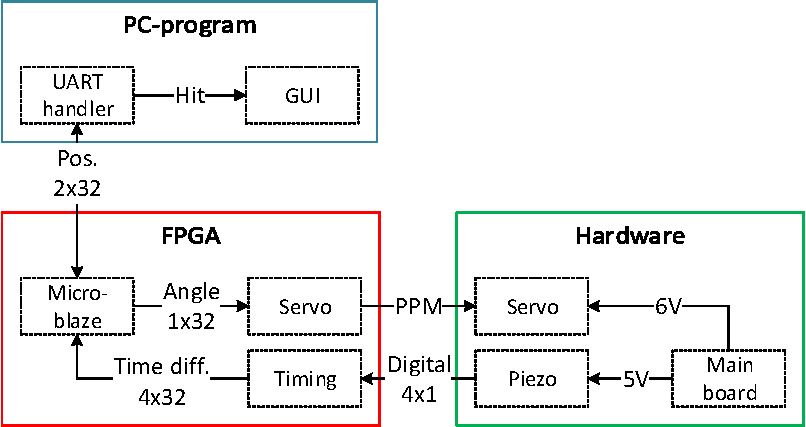
\includegraphics[width=1\textwidth]{figures/overview}
		\caption{Top level diagram of the combined system components with bus widths assigned.}
		\label{fig:overview}
	\end{figure}
	%
	Once a piezoelectric sensor triggers an input pin on the FPGA, the current system time is noted.
	When all four inputs have been triggered, the microprocessor receives an interrupt and begins finding the $(x,y)$-position of the impact point.
	The solution is used to actuate the arm and position it to catch the ball as it returns to the platform after the first bounce.
	
	The impact point is stored in microprocessor memory until the next ball-impact, and can be requested by the PC program through UART.
	Finally the GUI shows a visual interpretation of the data.
	%
	\section{Time difference of arrival (TDOA)}
	In this section the relationship between differences in time measurements from multiple sensors and the $(x,y)$-position of the emitter are derived.
	The problem can be modelled as in figure \ref{fig:tdoa_model} where the following parameters are constants given from the physical configuration and measurements:
	\begin{itemize}
		\item Time of arrival of sound at sensors $a$, $b$, $c$ and $d$.
		\item Speed of sound in chosen material.
		\item Position of sensors.
	\end{itemize}

	The system is set up with four sensors because the risk of obtaining multiple solutions when using only three \cite{tdoa_book}.
	The solution will be represented as a system of linear equations to enable fast and relatively simple implementation in C.
	The derivation will be conducted for two of the sensors, giving one row in the system of equations. The remaining two rows are determined in a similar manner.
	\begin{figure}[htb]
		\centering
		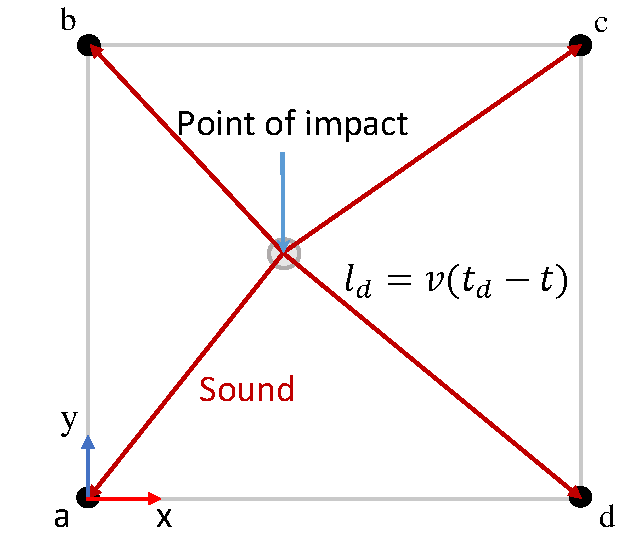
\includegraphics[width=.6\textwidth]{figures/tdoa_model}
		\caption{Top-down view of platform surface area showing sensors and impact point.}
		\label{fig:tdoa_model}
	\end{figure}
	%
	Assuming constant speed of sound through the impact plane, \eqref{eq:speedOfSoundDistA} describes the relationship between time difference between measurement and impact $(t_a - t)$ and the distance the impact point is from sensor $a$.
	\begin{equation}
		l_a = v(t_a - t) \Leftrightarrow l_a^2 = v^2(t_a - t)^2
		\label{eq:speedOfSoundDistA}
	\end{equation}
	Eq. \ref{eq:speedOfSoundDistB} describes the same relationship with respect to sensor $b$.
	\begin{equation}
		l_b = v(t_b - t) \Leftrightarrow l_b^2 = v^2(t_b - t)^2
	\label{eq:speedOfSoundDistB}
	\end{equation}
	By differencing \eqref{eq:speedOfSoundDistA} and \eqref{eq:speedOfSoundDistB}, \eqref{eq:distanceDiffRelativeToTime} can be derived using the difference of squares formula. It is a linear relation with respect to time of impact $t$.
	\begin{equation}
		l_a^2 - l_b^2 = v^2(t_a^2 - t_b^2) - 2 v^2 (t_a - t_b) t
		\label{eq:distanceDiffRelativeToTime}
	\end{equation}
	By using Pythagoras theorem the difference in squared distances from the impact point are also related according to \eqref{eq:distDifference}. It can be seen that it is a linear equation in x and y with constants given from the setup.
	\begin{equation}
		\begin{split}
			l_a^2 - l_b^2 & = (x_a - x_b)^2 + (y_a - y)^2 - ((x_b-x)+(-y_b - y))^2 \\
			& = -2( (x_a - x_b) x + (y_a - y_b) y ) + x_a^2 +y_a^2 -(x_b^2 + y_b^2)
		\end{split}
		\label{eq:distDifference}
	\end{equation}
	By setting \eqref{eq:distanceDiffRelativeToTime} and \eqref{eq:distDifference} equal and isolating the constants known from time measurements and setup, \eqref{eq:firstRow} is derived.
	\begin{equation}
		(x_a - x_b) x + (y_a - y_b) y - v^2(t_a - t_b) t = (x_a^2 +y_a^2 -(x_b^2 + y_b^2) - v^2(t_a^2 - t_b^2))/2 \equiv k_{ab}
		\label{eq:firstRow}
	\end{equation}
	Using similar relations for the other four sensors results in the system of linear equations \eqref{eq:linsys} which solution uniquely defines the $(x,y)$-position of the impact point \cite{tdoa_notes}.
	\begin{equation}
		\begin{bmatrix}
			x_a - x_b & y_a - y_b & - v^2(t_a - t_b) \\
			x_b - x_c & y_b - y_c & - v^2(t_b - t_c) \\
			x_c - x_d & y_c - y_d & - v^2(t_c - t_d)
		 \end{bmatrix}
		 \left[ \begin{array}{c} x \\ y \\ t \end{array} \right] = \left[ \begin{array}{c} k_{ab} \\ k_{bc} \\ k_{cd}\end{array} \right]
		 \label{eq:linsys}
	\end{equation}
% chapter overall_design_priciples (end)
	\chapter{Mechanics} % (fold)
\label{cha:Mechanics}
	When the ball is dropped has to be picked in the first bounce. 
	For this, a mechanical structure holds an actuator that moves an arm which takes the ball according to the data from the FPGA.

	\section{Design} % (fold)
	\label{sec:design}
		The physical implementation of the project is divided in three parts.

		First, the platform where the sensors are allocated. 
		The physical platform area will be a flat area of approximately $40\times40\,\si{\centi\meter}$.
		This platform was decided to be an aluminum sheet due to two reasons: metal sheets usually have homogeneous mechanical properties and this especially important for this project because the same propagation waves speed is searched; and, inside the metals, aluminum was choosen for stock reasons and easy manufacturing. 
		This platform is separed from the down surface with a plastics legs ij the corners that let the waves, first reach the sensors and then dissipate through them.

		Second, a structured has to be design for hold the motor and the arm. 
		This has been designed so it lets the user to change the height of the actuator for test the machine in different conditions. 
		This capability will be used to measure the reaction speed of the project. 
		Also, the structure has to be strong and rigid enough to doesn't deform more than an specified precision.

		Third, the actuator will let move an arm that will take the ball when required. 
		This actuator needs to be precise enough to satisfy the precision criteria of the project. 
		The arm was decided to have only one motor for simplicity reasons and as a prove of concept. 
		The inverse cinematics is really easy to calculate and is much simpler in the assembly and maintenance.
			
	% section design (end)

	\section{Inverse kinematics and control }
	\label{sec:kinematics}
		The inverse kinematics for the one joint arm can be calculated very simple using the x and y position calculated from the TDOA information using equation \ref{eq:angle}.

		\begin{equation}
			angle = atan(y/x)
			\label{eq:angle}
		\end{equation}

		This calculation are easily implemented in c code on microblaze MCS.

		\subsection{Servo control}
		The servo are controlled to move the arm to the calculated angle. By testing it is found that the servo copes with the standard for servos by going to zero degree when a $1\si{ms}$ high is applied. When the PPM signal is high for $2\si{ms}$ it moves to a $90\si{\degree}$ angle. In between there are a linear relationship between the time with high signal and the amount of degrees it moves to.
		Todo: finish this, maybe change implementation in VHDL
		The amount of time the servo is high are controlled with the generic PWM module designed in project one which recessives the number of

		%The PWM generator is a rather simple component which outputs a square signal with the desired period and variable duty cycle.
		%The implementation has generic parameters for in- and output frequencies which enables the user easily instantiate a component with the correct output signal period.

		%Duty cycle resolution is also specified upon instantiation, allowing for more or less fine-grained control of PWM duty cycle.
		%For example, a resolution of two bits allows selection of the duty cycle steps $0, 33, 66$ and $100\%$.

	\section{Inverse kinematics and control}
	%\label{kinematics}
		Due to the construction of this prototype with just one servo, the position of the servo is defined by:

		$$\theta = \arctan\frac{y}{x}$$

	\section{Manufacturing} % (fold)
	\label{sec:manufacturing}
		Due to the requirement to make the structure with differents positions to allocate the motor, the size of it implies manufacture it with the laser cutting technology. 
		The available let make big parts up yo 800mm 
	% section manufacturing (end)


	\section{Conclusions} % (fold)
	\label{sec:mec_conclusions}

	% section conclusions (end)

% chapter chapter_name (end)
	\chapter{Electronics} % (fold)
\label{chap:electronics}
This chapter describes the construction of a number of sensor circuits using piezo electric elements to measure the time of arrival of bending waves.
\section{Design of comparator circuit for the piezo electrics elements}
This section describes the construction of a number of sensor circuits using piezo electric elements to measure the time of arrival of bending waves.

There is a circuit like the one on figure \ref{fig:print} for each sensor. It is chosen to make one print for each circuit in order to keep the wires conducting the analog sensor values as small as possible.
\begin{figure}[htb]
	\centering
	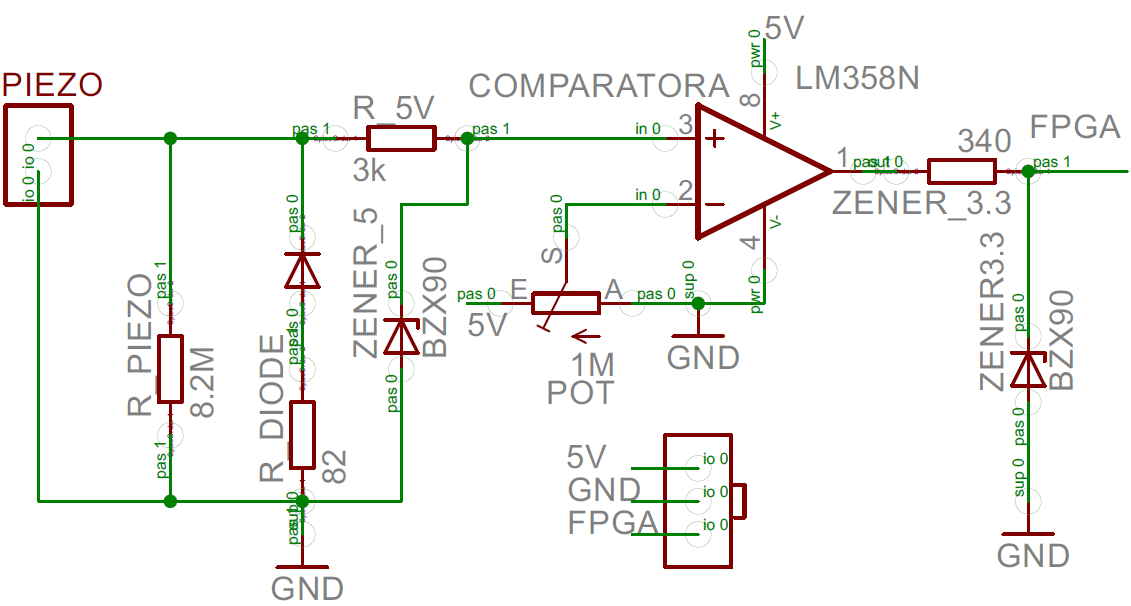
\includegraphics[width=.8\textwidth]{figures/Print}
	\caption{Schematics of circuit for digitalizing the output from a piezo electric elements.}
	\label{fig:print}
\end{figure}
The very small current that the piezo electric element generates are amplified with a resistor on $8.2\si{\ohm}$. This value is chosen since test showed that it was possible to detect ball bounce after a drop from a hight on $30\si{\centi\meter}$ which are deemed as the minimum drop hight.
Diodes are used to account for the large positive and negative voltage spikes that the sensor in combination with the large resistor can output in case of a powerful input to the sensor.
Since the negative voltage are not use it is removed up to $0.7V$ with a diode which conducts current from ground when the voltage from the piezo becomes less then $0.7V$.
The resistor to limit this current is calculated according to equation \ref{eq:distDifference}.
\begin{equation}
20 - 0.7 V = R_{diode} \cdot 300mA \Leftrightarrow R_{diode} = 64.3\si{\ohm}
\label{diodeResistor}
\end{equation}
The $20V$ is taken as a guess on the absolute maximum based on the fact that tests has not shown voltages above $15V$ when throwing the ball against the plate. Hence the system are robust against misuse. A resistor with a value above and close to $64.3\si{\ohm}$ that are available in stuck are used.
Since the op-amp cannot compare values that are larger than the supply of $5V$, the positive voltage is limited to $5.1V$ with a zener diode \cite{zener}. The resistor $R_5V$ is calculated by assuming infinite input resistance in the op-amp according to equation \ref{eq:zener5VResistor}.
\begin{equation}
%20 - 5 V = R_{5V} \cdot 5mA \Leftrightarrow R_{diode} = 3{k\si{\ohm}
\label{eq:zener5VResistor}
\end{equation}
A zener diode \cite{zener} is used to convert the $5V$ on the data output from the operational amplifier to $3.3V$, which is appropriate voltage for the FPGA. The solution with a zener diode is chosen over a another using a voltage divider since the voltage is kept at $3.3V$ for all op-amp's of the type LM358 even in cases of changes in production. According to the datasheet for LM358 the saturated output voltages varies from the supply voltages down to $1.5V$ below \cite{lm358}.
The resistor placed on the output of the operational amplifier is calculated using the current used for testing conditions in the datasheet for the diode, as can be seen in equation \ref{eq:zener} \cite{zener}.
\begin{equation}
5-3.3V = R_{z} I_{test} \Leftrightarrow R_{z} = 1.7V/5mA = 340\si{\ohm}
\label{eq:zener}
\end{equation}
%
A potentiometer is connected to the inverting pin of the op-amp in order to ease the tuning of the reference voltage. It's value is set to $1\si{\mega\ohm}$ to minimize the power consumption.
The tuning of the reference voltage is conducted by dropping a ball from $30\si{\centi\meter}$  and that the comparators are triggered. The voltage are lowered until the one off the sensor circuits does not detect the ball hit. Then it is raised to a bit above that to ensure detection. Hence the reference voltage for all of the four circuits are adjusted to $9.4V$ which have proven to be very robots against disturbances in the form of vibrations in the surrounding while still being able to detect ball hits.
%
\subsection{PCB Design and manufacturing}
After designing the schematics it was verified on a breadboard. Then the design from the breadboard are drawn as a schematics and a board in eagle.
The PCB is routed to keep wires as short as possible in order to minimize influence of noise as can be seen on figure \ref{fig:pcb}.
\begin{figure}[htb]
	\centering
	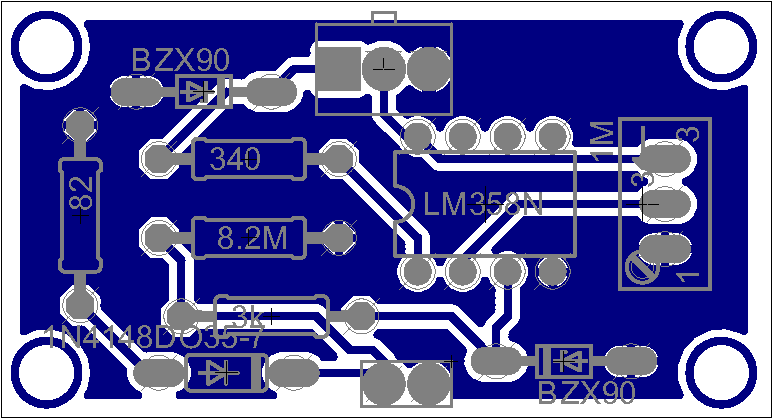
\includegraphics[width=.6\textwidth]{figures/pcb}
	\caption{PCB board of circuit for digitalizing the output from a piezo electric elements.}
	\label{fig:pcb}
\end{figure}
The width of the wires are chosen to be thick in order to ease the manufacturing. Then the risk of the wires disappearing in the basic fluid are smaller.
After verifying the schematics one of the four identical PCB's are manufactured and tested before producing the others.
Other simpler electrical connections are manufactured on stripboards to minimize time spend on producing PCB's.

	\chapter{Low Level Programming} % (fold)
\label{chap:low_level_programming}

    %!TEX root = ../../report.tex
\section{Digital design}
\label{cha:digidesign}

To accurately measure when each piezoelectric sensor has an impact, %spelling??
a timing module is implemented in VHDL.
The timing module takes each piezoelectric sensor as an input and measures the time between each sensor registers the ball impact.
This time information may then be used to solve for the $(x,y)$ position of the impact point of the ball.

Because solving the resulting system of equations in hardware directly is deemed rather hard, %reference?
 a MicroBlaze soft core is made part of the hardware design for the FPGA.

 Full RTL and technology diagrams generated by the Xilinx tools may be found in Appendix \ref{cha:digi-diagrams}.

\subsection{Timing module}
\label{sec:timing_module}
The timing module has a separate input for each of the four piezoelectric elements.
Each input is attached to an SR latch synchronised with the FPGA 50\si{MHz} clock so that input signals are sampled every 20\si{ns}.

\begin{figure}[htb]
    \centering
    %!TEX root = ../report.tex
\begin{tikzpicture}[every path/.style={},>=triangle 45]
    \def\srlatch(#1)#2#3{%
      \begin{scope}[shift={(#1)}]
        \draw (0,0) rectangle (1,1.5);
        \node at (0.75,1.25) {$Q$};
        \node at (0.75,0.25) {$\overline{Q}$};
        \draw (1,1.25) -- +(0.25,0) coordinate (#2 Q);
        \draw (0,0.25) node[right] {$S$} -- +(-0.25,0) coordinate (#2 S);
        \draw (0,0.75) node[right] {$C$} -- +(-0.25,0) coordinate (#2 C);
        \draw (0,1.25) node[right] {$R$} -- +(-0.25,0) coordinate (#2 R);
      \end{scope}
    }

    \srlatch(0,0){a}{$Q_0$}
    \srlatch(2.5,0){b}{$Q_1$}
    \srlatch(5,0){c}{$Q_2$}
    \srlatch(7.5,0){d}{$Q_3$}

  % Connect all the K and J ports
  % \draw (a K) to[short,-*] (a J);
  % \draw (b K) to[short,-*] (b J);
  % \draw (c K) to[short,-*] (c J);
  % \draw (d K) to[short,-*] (d J);

  % % Connect the T ports to the incoming signal
  % \draw (-1,-1) node[ocirc,label={left:$E$}] (E) {};
  % \draw (a T) -- ++(-0.2,0) coordinate (inter) -|
  %   (E -| inter) node[circ] {};
  % \draw (b T) -- ++(-0.2,0) coordinate (inter) -|
  %   (E -| inter) node[circ] {};
  % \draw (c T) -- ++(-0.2,0) coordinate (inter) -|
  %   (E -| inter) node[circ] {};
  % \draw (d T) -- ++(-0.2,0) coordinate (inter) -|
  %   (E -| inter) node[circ] {} -- (E);
  % % Place the bits and the +
  % \draw[->] (a J) -- ++(0,1) node[left] {$+$};
  % \draw (a Q) to[short] ++(0,2) node[ocirc,label={left:Bit 0}] (bit0) {};
  % \draw (b Q) to[short] ++(0,2) node[ocirc,label={left:Bit 1}] (bit1) {};
  % \draw (c Q) to[short] ++(0,2) node[ocirc,label={left:Bit 2}] (bit2) {};
  % \draw (d Q) to[short] ++(0,2) node[ocirc,label={left:Bit 3}] (bit3) {};
  % % AND ports
  % \draw (c J) |- ++(-0.2,0.5) node[and port] (c and) {};
  % \draw (d J) |- ++(-0.2,1.5) node[and port] (d and) {};
  % % Output connections
  % \draw (b J) to[short,-*] (a Q);
  % \draw (c and.in 2) to[short,-*] (c and.in 2 -| bit1);
  % \draw (c and.in 1) to[short,-*] (c and.in 1 -| bit0);
  % \draw (d and.in 2) to[short,-*] (d and.in 2 -| bit2);
  % \draw (d and.in 1) to[short,-*] (d and.in 1 -| bit0);
  % % I had to guess this connection, because the and port doesn't
  % % have additional anchors
  % \draw ($(d and.in 2)!0.5!(d and.in 1)+(0.4,0)$) coordinate (help)
  %   to[short,-*] (help -| bit1);
\end{tikzpicture}

    \caption{Timing module logic diagram.}
    \label{fig:timing}
\end{figure}

The timing module continuously counts the number 50\si{MHz} clock cycles elapsed.
When an input signal is detected, the SR latch is set and the number of clock cycles elapsed at that time is saved to a register.
Time is saved to a different register once per piezoelectric sensor input edge.

When all four SR latches have been triggered, the timing module calculates the time difference between the input that was triggered first and the remaining three.
The output is thus four 32-bit values, where at least one is always zero -- namely the first one triggered.
The line \custtt{timings\_ready} is pulled high when all four inputs have been triggered and corresponding time values recorded.
The \custtt{timings\_ready} signal is attached to an external interrupt on the MicroBlaze microprocessor.

After one read-cycle of four triggered input signals, the timing module is in a \emph{hold}-state until it has been reset by pulling its \custtt{reset} signal high.
The microprocessor is responsible for resetting the module.

% delays introduced

\subsection{MicroBlaze soft microprocessor}
TODO (merge w/ Anders)

\subsection{Servo control?}
PWM duty to angle value?


	\section{Microblaze MCS}
A Microblaze micro controller system(MCS) is used for handling the following tasks in descending priority:
\begin{itemize}
	\item Fast and precise solution to the TDOA problem.
	\item Calculating inverse kinematics for the robot arm.
	\item Handling UART communication with a PC.
\end{itemize}
The choice of using a MCS is due to expediency in the implementation.
%
\subsection{Setup of Microblaze IP-core} 
It is chosen to implement the solution of the TDOA problem in Microblaze MCS version 1.4. This soft core microcontroller implemented on an FPGA is used rather than developing the solution directly in VHDL. 
The reason for this choice is that it is easier to implement the commonly used numerical methods for solving systems of linear equations in a sequential order rather than in parallel. 
The smaller and older Picroblaze MCS is avoided since xilinx does not support a C compiler  
($http://forums.xilinx.com/t5/PicoBlaze/PicoBlaze-FAQ-Is-there-a-C-Compiler/td-p/580$). 
The Microblaze system with more than 4k of memory has proven take up more than the 50K logic gates available on the XC3S50AN, that is mounted on the previously use development board ($http://www.xilinx.com/support/documentation/data_sheets/ds557.pdf$). 
This small memory size is too small for easy implementations which often includes large programs. As an example of a nice function that takes op a lot of program space is the printf function, that is very useful for debugging.
Due to these limitations the more suitable Nexus 2 board is used which includes an Spartan-3E with 500K gates.  
%
The Microblace MCS is included in the VHDL project as an IP-core using the IP-core generator GUI in ISE-design suit. Here the settings are left at their default values unless otherwise needed. The memory size is assigned to 32k since test showed sufficient space on the FPGA for this. The UART is setup to transmit and recive at a baud rate on 115200 without using interrupts. Four general purpose inputs(GPI) with a size of 32 bits is used to receive four timings values. The 32 bits precision is used since the Microblaze has a is a 32-bits processor. Two general purpose outputs(GPO) is used. One of them contains the newest calculated angle from the inverse kinematics and the other one is used as a flag indicating that a new angle is available. One external interrupt is used to initialize the calculation of the TDOA problem. 
%
\subsection{C-program on Microblaze}
The program running on the Microblaze is built op rather simple with a setup sequence followed by a while true loop responding with results of the TDOA problem upon request from the PC-program. Since there is rather strict timing constrains on calculating the inverse kinematics in order to move the arm under the ball before a second hit, the calculations are handled in a interrupt service routine. After the calculations are done a software timer is started. When the time have elapsed the timing measurements are enable again by setting a flag through a GPO port and the servo angle are set to its default position. The program is build using standard math utilities and specialized Microblace tools for GPIO, interrupts and UART.
%
\subsection{Interrupts on Microblaze}
The code in listing \ref{lst:interrupt} enables external interrupts by adding an interrupt handling routine that handles the calculations to the external interrupt 1.
%
\begin{lstlisting} [float={htb}, language=C, caption={C code that enables external interrupt},label={lst:interrupt} ]
microblaze_register_handler(XIOModule_DeviceInterruptHandler,XPAR_IOMODULE_0_DEVICE_ID);
XIOModule_Connect(&gpio, INTR_ID1, (XInterruptHandler)isr, XPAR_IOMODULE_0_DEVICE_ID);
XIOModule_Enable(&gpio, INTR_ID1);
microblaze_enable_interrupts();
\end{lstlisting}
It does this by first registering the devices interrupt handler that handles all interrupts. After that the interrupt routine; isr, are added to the interrupt table and bounded to the interrupt id for interrupt 1. Lastly the interrupts is enabled by firstly enabling the interrupts for interrupt 1 and afterward enabling interrupts globally.
%
\subsection{Solve TDOA}
The solution to the TDOA problem is handled by solving the system of linear equations described in section TODO:(intro about TDOA reference). To keep implementation simple the solution is implemented with gauss elimination. Software implemented floating point precision are used in the calculations due to the fact that the used free version of Microblaze does not include a floating point arithmetic unit. 
The gauss elimination is implemented by running through each column and for each do the following \cite{gauss}:
\begin{itemize}
	\item Pivoting by sorting the from top to bottom rows according to descending pivot elements.
	\item Eliminate elements in column under current pivot element by subtracting the current row multiplied with the element in the pivot column under the pivot element under consideration divided with the pivot element.
\end{itemize}
When the iterations reaches the last column the coefficient matrix is on an upper triangular matrix form. This enables back substitution starting from the button row and calculating the solution x based on the previous calculated solution as can be seen in equation.
\begin{equation}
	x_n = \frac{b_n}{a_{nn}}
\end{equation}
%
\begin{equation}
	x_i = \frac{1}{a_{ii}} (b_i - \sum_{j=i+1}^{n-1} a_{ij}x_j)
\end{equation}
Where a is the coefficient matrix, b is the right hand side vector and n is the number of rows and columns.
%
The inverse kinematics are calculated using $atan(y/x)$ where $y$ and $x$ are the calculated coordinates of the impact point. 
%
\subsection{GPIO and UART}
The reading from general purpose registers are done using the command
\custtt{XIOModule\_DiscreteRead(\&gpio, \#GPO register)}
Where the gpio is a struct handling the IO's that are initialized and started before use.
Writing to a GPO is done in a similar way.
By running the command \custtt{XIOModule\_CfgInitialize(\&gpio, NULL, 1)} the reading from the UART is enabled.

\section{Inverse kinematics and control }
\label{sec:mechanics_kinematics}
The inverse kinematics for the one joint arm can be calculated very easily using the x and y position calculated from the TDOA information using equation \ref{eq:angle}.

\begin{equation}
\theta = atan(y/x)
\label{eq:angle}
\end{equation}

This calculation are easily implemented in C code on microblaze MCS.

\subsection{Servo control}
The servo is controlled to move the arm to the calculated angle. By testing it is found that the servo copes with the standard for servos by going to zero degree when a $1\si{ms}$ high is applied. When the PWM signal is high for $2\si{ms}$ it moves to a $90\si{\degree}$ angle. In between there is a linear relationship between duty cycle and the degrees it moves to.
%
\subsection{Evaluation}
The ability of the implemented programs ability to for fill the tasks it is assigned to have been verified separately. The correctness of the solution of the implemented Gauss-elimination have been verified by comparing solutions with MATLAB's solution which give precisely the same solution.

% chapter low_level_programming (end)

	\chapter{High Level Programming}
\label{chap:high_level_programming}
	A computer program will show the position of the hit point
	\section{Communication and Logic}
	\label{sec:communication_and_logic}
		Regarding the communication, the computer program and the FPGA are connected by a USB cable and this protocol is handle by the qt serial libraries given.
		This enables communication using code that has already been tested.

		The program is the master in the communication, and it tries to establish communication by default from the beginning.
		While there are a default connection options, a settings window has been implemented so the user can change the options easily.
		This options are: $Baud Rate, Parity, Stop Bits, Flow Control$ and $Local Echo$.

		Once the communication is establish, the program sends a character that the FPGA interprets as $send hit information$.
		Then, the FPGA sends through the USB the $x$ and $y$ coordinated along with a $hash$ of the hit, that defines a unique identifier for it.
		If the hit is a new hit, the program shows it in the UI and saves it in the history so that the user can see them again when desired.
	\section{Interface}
	\label{sec:program_interface}
		The UI has been developed so the user can easily configure the connection and see the hits.
		On one hand, the connection is establish automatically from the start, so the user does not need to do anything. Furthermore the hits, are immediately shown in an intuitive square that represents the platform where the sensors are located.

		On the other hand, the interface only has two buttons. The first one is $Settings$ and it opens a window where the connections parameters can be configured. The second is $History$ and, when clicked once, it shows all the hits positions in that session. If clicked again, the program come back to detect more hits.

		In summery, the program implements a pretty and easy to use interface between the machine and the user giving the opportunity to all kind of users being able to use it. Furthermore it stores a graphical history for further researches.

	\section{Conclusions} % (fold)
	\label{sec:high_level_programming_conclusions}
		After having carried out all the experiments and tests we can assure the interface is not just stable and reliable, but also really easy to use.
		The UI has shown to be both simple and useful when the test were made and also the connection has always been easy to set up from the beginning.
		The program has been written in Qt and hence it is multi platform and we have had the opportunity to test it out in a Windows and Ubuntu based computers giving the same results.
	% section conclusions (end)
		\begin{figure}[htb]
			\begin{center}
				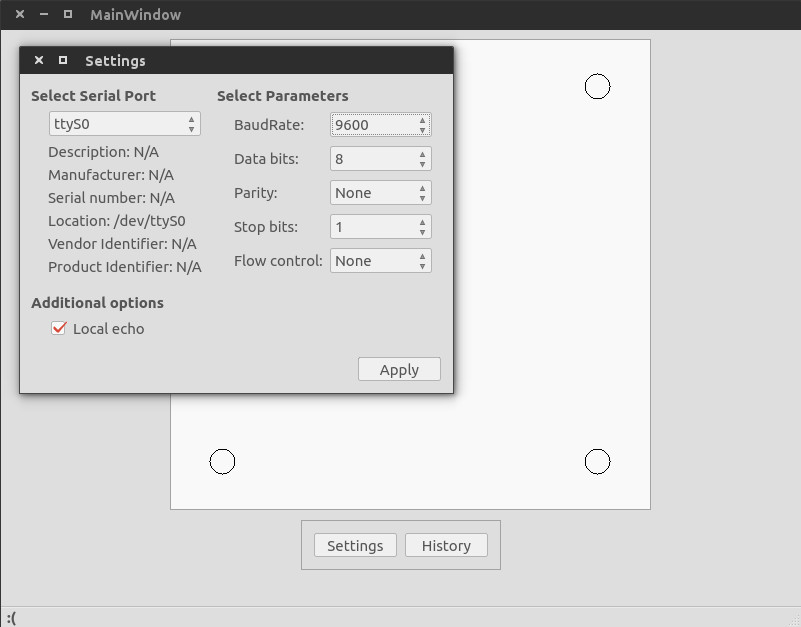
\includegraphics[width=.8\textwidth]{figures/UI}
			\end{center}
			\caption{UI of the program}
			\label{fig:ui}
		\end{figure}

	\chapter{Experiments} % (fold)
\label{chap:experiments}
In this chapter the validation of the ping pong ball catchers ability to determine the point of impact on the base plate and being able to move to catch the ball after a ball bounce back.
\section{Catching the ball in time}
In order to validate that the calculations and movement of the servo is fast enough to catch a ping pong ball after a bounce back after a drop from $30\si{\centi\meter}$. The ping pong ball is dropped over the center of the plate, where the positioning system often calculates the impact point to be. The arm goes in and catches the ball in without troubles. 
Based on this result it is concluded that the timing constrains on calculating where the arm should move to and moving it there are satisfied.
\section{Positioning}
In order to test whether the positioning system calculates the correct position tests were conducted.
In each test a ball is dropped on to the same position on the base plate. The target is 30 degrees from the x-axis and a distance of the arms length from the origo. This target is marked with a red dot on figure \ref{fig:testRes30deg}. 
As can be seen in the figure the positions of the impact points are calculated to be at very different places at the different attempt of dropping the ball at almost the same point.
\begin{figure}[htb]
	\centering
	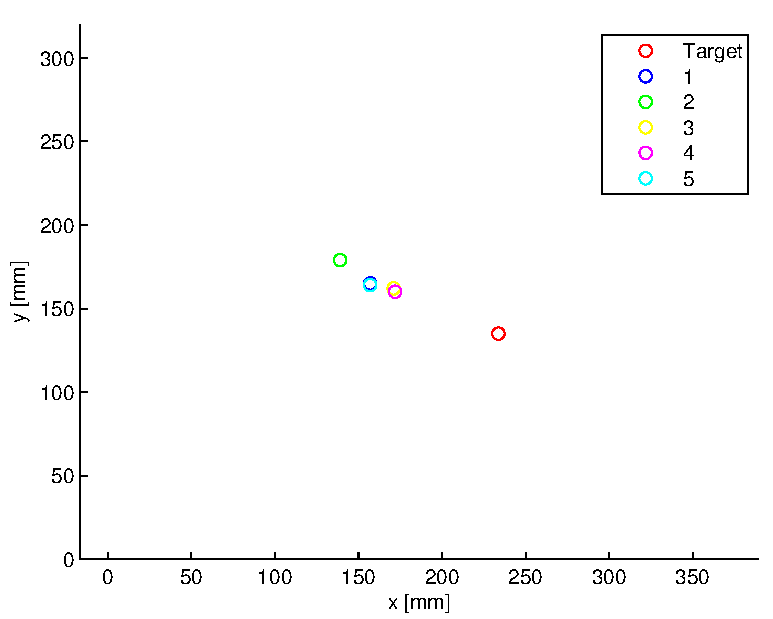
\includegraphics[width=.8\textwidth]{figures/testRes30deg.pdf}
	\caption{Estimated impact positions based as a result of dropping a ball on to the same target multiple times.}
	\label{fig:testRes30deg}
\end{figure}
The reason to this error is differences in the timings as can be seen in figure \ref{fig:clockCycles30deg}. In the figure the time difference between the four measurements on respectively sensor a, b, c and d. Which is indicated as blue, cyan and yellow. The measurements on d cannot be seen since they are zero for all the measurements. As can be seen the measurements are all over the place.

\begin{figure}[htb]
	\centering
	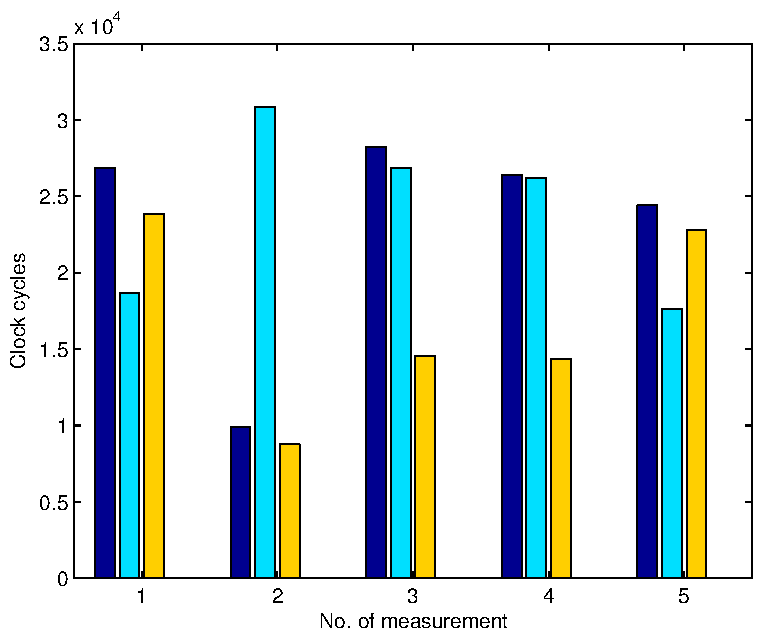
\includegraphics[width=.8\textwidth]{figures/clockCycles30deg.pdf}
	\caption{Estimated impact positions based as a result of dropping a ball on to the same target multiple times.}
	\label{fig:clockCycles30deg}
\end{figure}

\section{Unstable to small changes in time}
To validate the timings the timing results from the timing VHDL component are compared with time difference calculated based on sampling the same sensor output on an oscilloscope. The sensor output can be seen on figure \ref{fig:timingPlot}. 
\begin{figure}[htb]
	\centering
	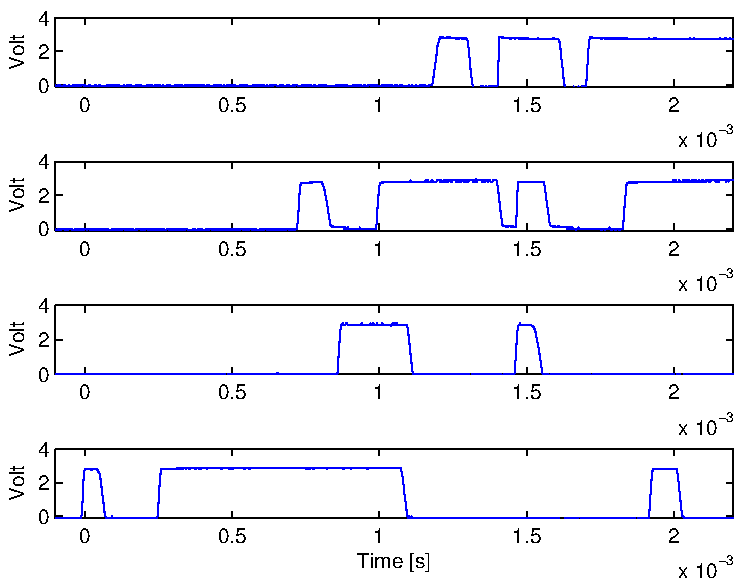
\includegraphics[width=.8\textwidth]{figures/timingPlot.pdf}
	\caption{Estimated impact positions based as a result of dropping a ball on to the same target multiple times.}
	\label{fig:timingPlot}
\end{figure}
Timings to compare with are extracted by running through the sequence from the beginning until a value larger than the 2.4V are reach. The time at these points are stored for each sensor. The compare time values in table \ref{tbl:compareCycles} can be calculated by multiplying the time difference between each of the stored times and the smallest of them with the clock frequency the timing component counts with(50Mhz). 
%
\begin{table}[h]
	\begin{tabular}{|l|l|l|l|l|}
		\hline		
		 & ta & tb & tc & td \\
		 \hline		
		Difference in cycles from timing module & 36655 & 59827 & 43481 & 0 \\	
		 \hline
		Difference in cycles from oscilloscope & 36600 &  60000 &  43400 & 0 \\		
		\hline				
	\end{tabular}
	\caption{Comparison of clock cycles from timing module and calculated from oscilloscope data.}
	\label{tbl:compareCycles}
\end{table}
%
As can be seen from table \ref{tbl:compareCycles} the compare values are roughly the same. Hence it is concluded that the timing is correct, so the fault must be before the FPGA in the system.
% chapter experiments (end)
	\chapter{Discussion} % (fold)
\label{cha:discussion}

% chapter discussion (end)
	\chapter{Conclusions}
\label{chap:conclusions}

	After the design, implementation of the project and have carried out all the experiments to determine the reach of the machine we are able to conclude that:
	\begin{itemize}
		\item Despite the 
	\end{itemize}

	%\nocite{*} %To print the no referencered referencies
	\printbibliography[heading=bibintoc]

	\appendix
		\chapter{Mechanical drawings}
		\label{chap:mechanical_drawings}
			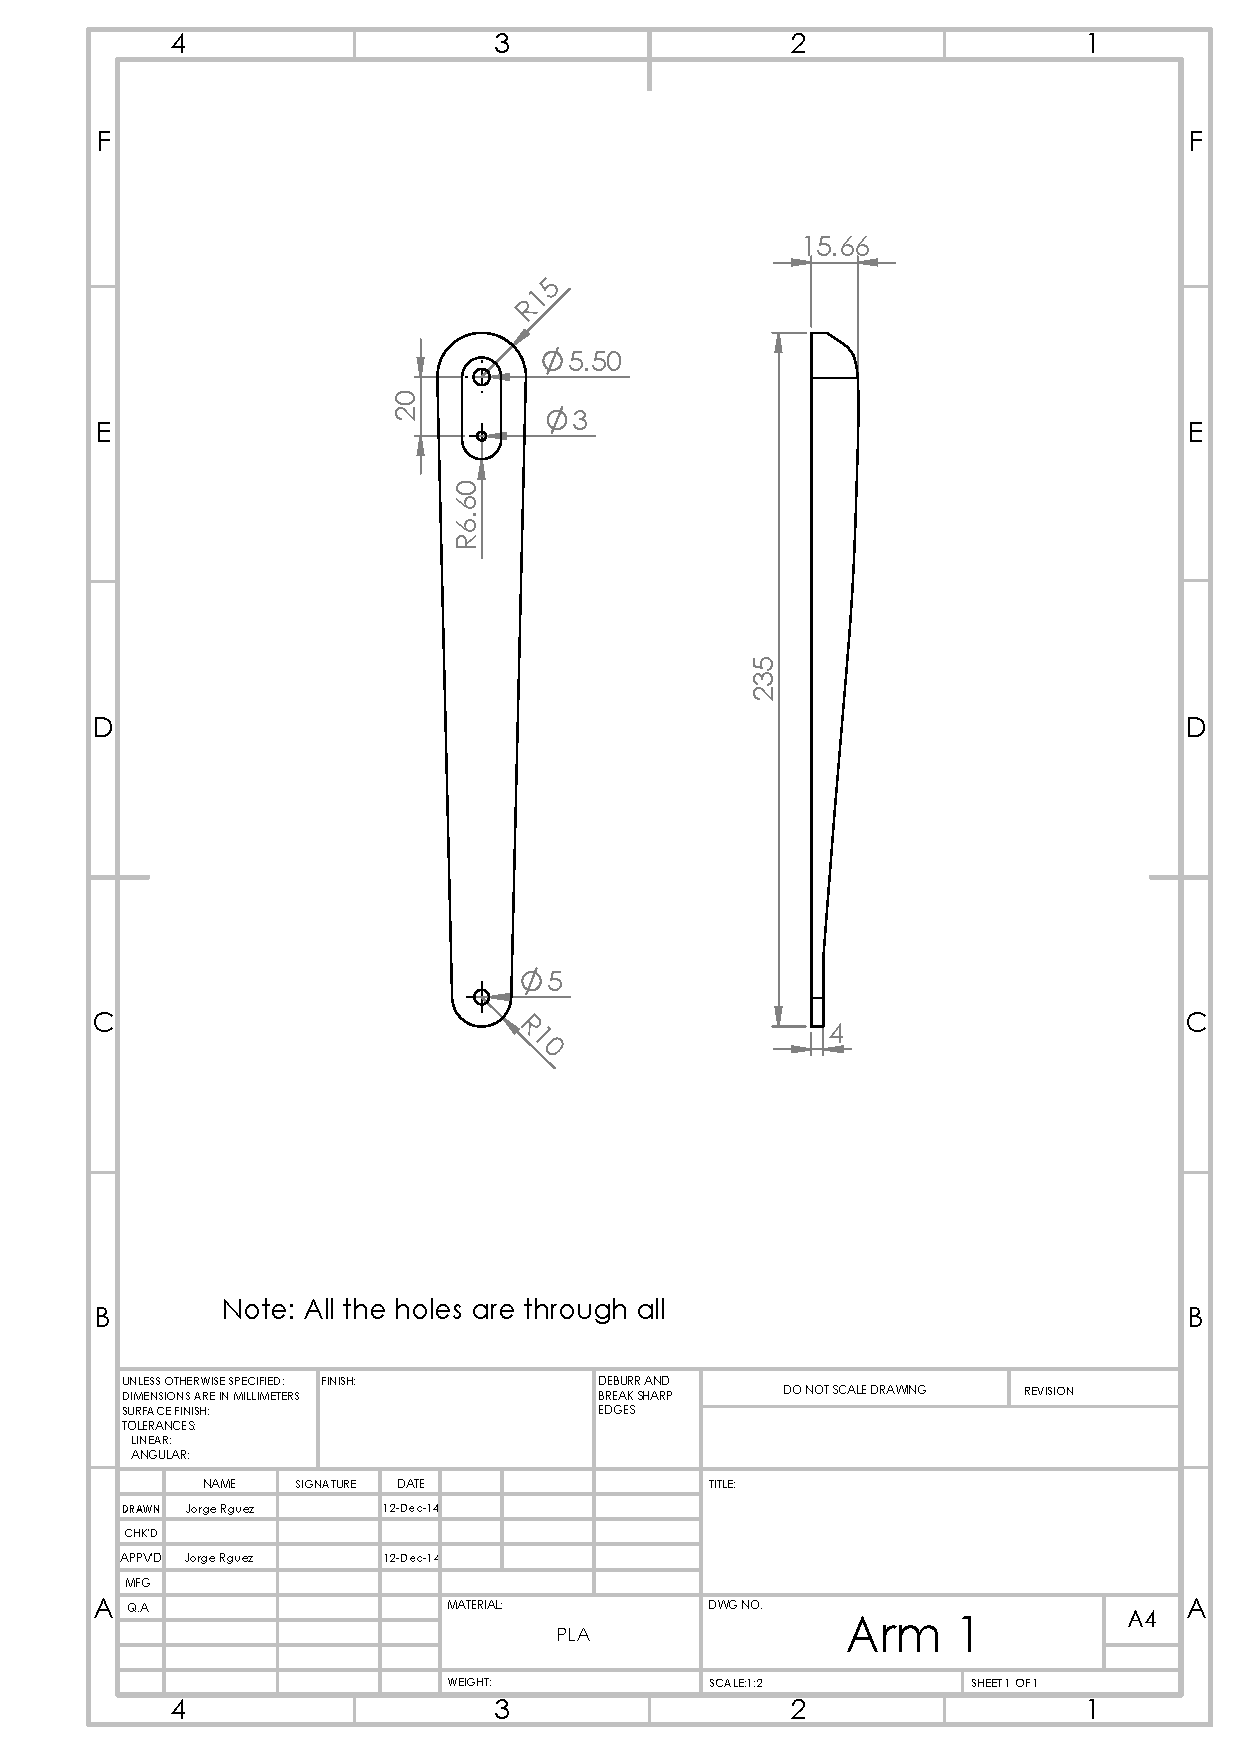
\includepdf[pages={1-7}]{includes/planes.pdf}

		\chapter{Digital circuit design diagrams}
		\label{chap:digi_diagrams}
			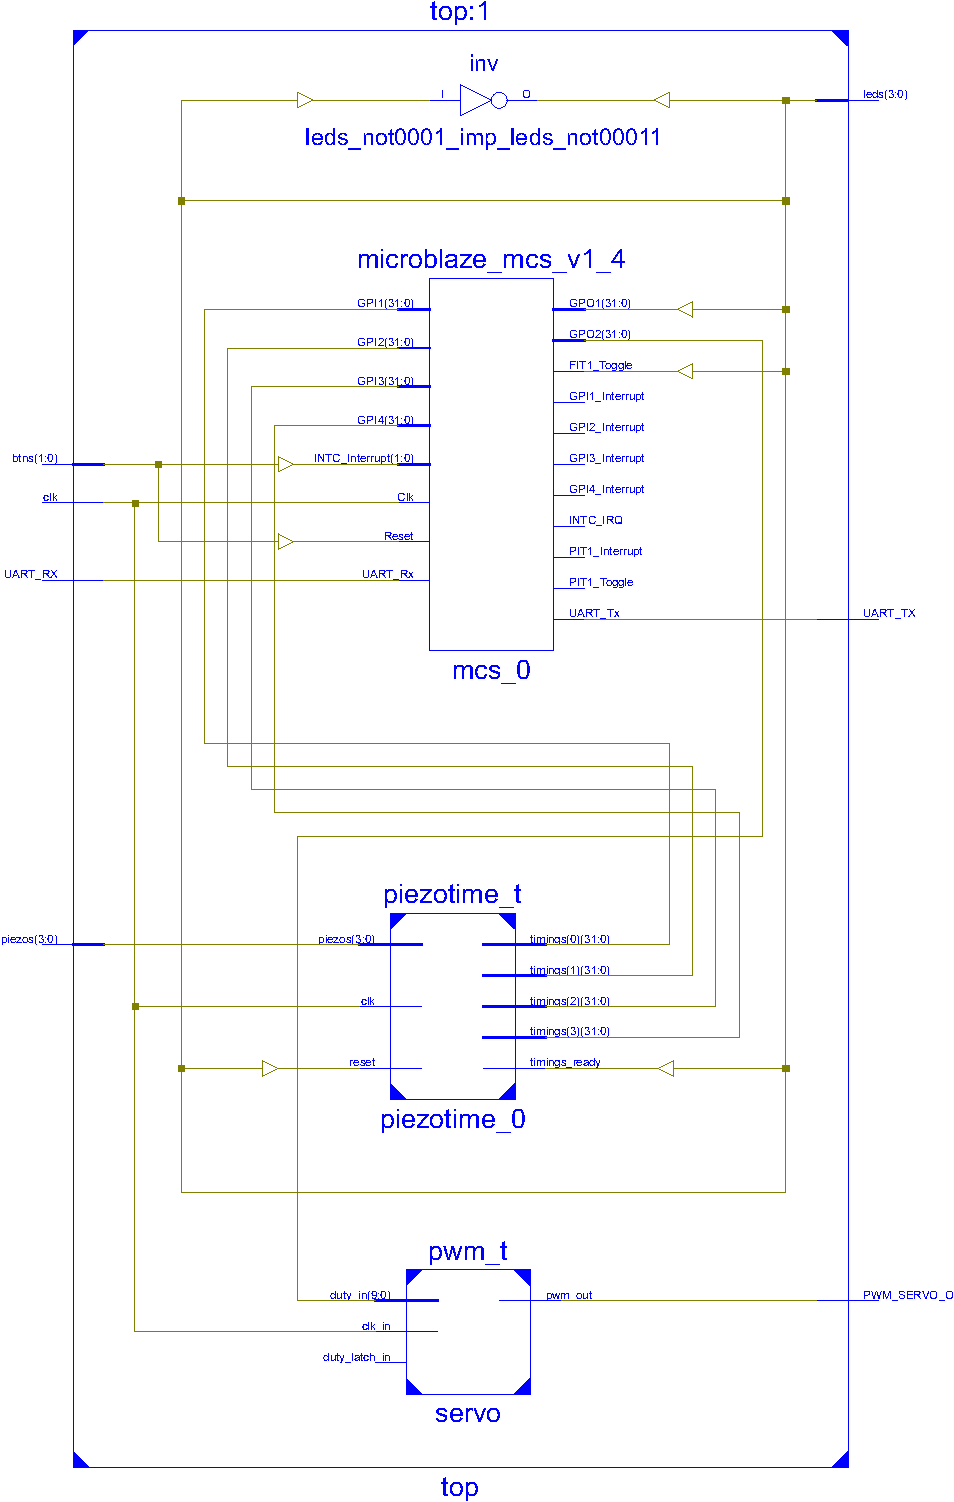
\includepdf[]{figures/rtl-sch.pdf}
			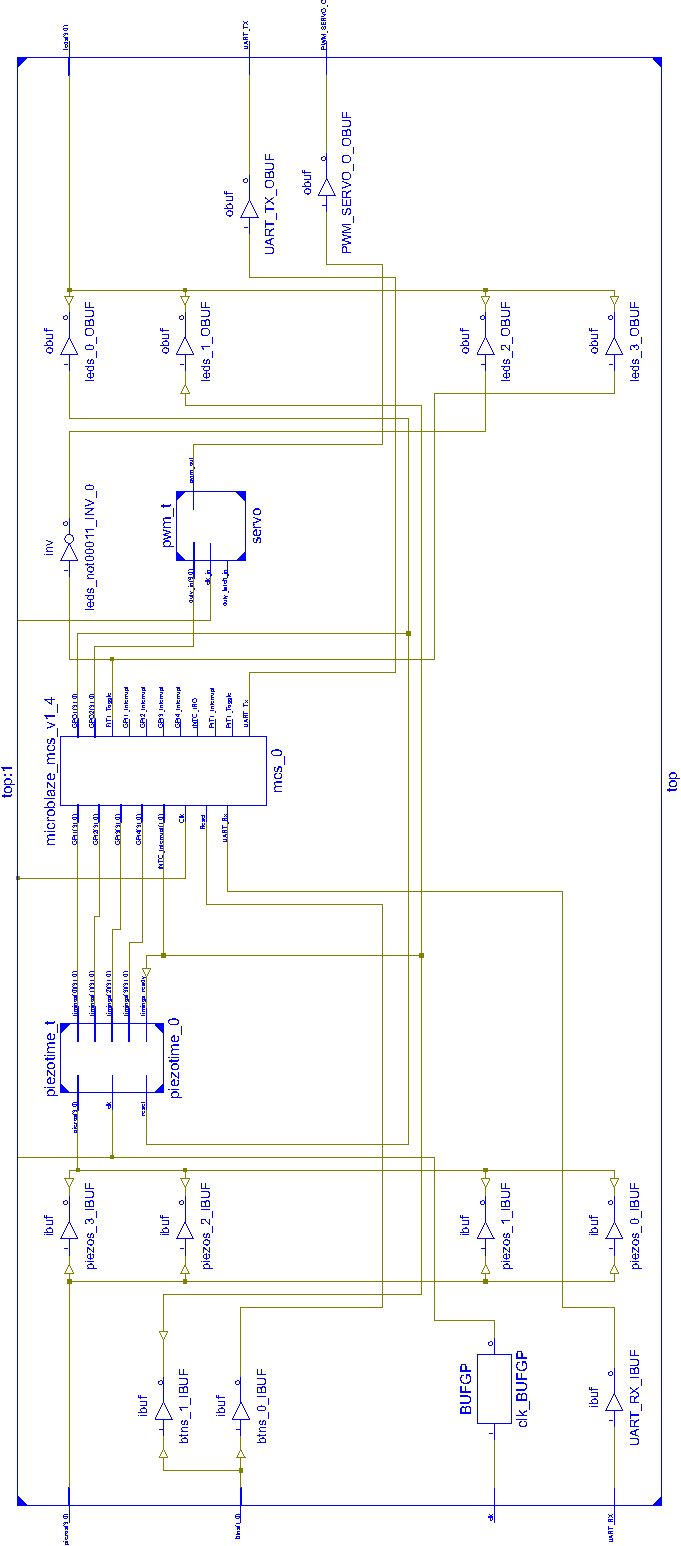
\includepdf[]{figures/tech-sch.pdf}

		\chapter{Equipment}
		\label{chap:equipment}
			To develop and test the designed solution the following equipments were used:
\begin{itemize}
	\item Oscilloscope
	\item Multimeter
	\item Soldering iron
	\item FPGA Spartan-3E on a NEXYS 2 board
	\item Eagle 7.1 Light
	\item Breadboard
	\item PCB development instruments
	\item Printer
	\item One DC servo motor
	\item Four murata piezo sensor 7BB-20-6L0
	\item 3D printer
	\item Laser cutter machine
\end{itemize}

\end{document}